\documentclass[c,8pt,xcolor...,x11names,usenames,dvipsnames]{beamer}
\usepackage{icclslides}
\usepackage[utf8]{inputenc}
\usepackage[british]{babel}
\usepackage{amssymb}
\usepackage{latexsym}
\usepackage{rotate}
\usepackage{tikz}
\usepackage{verbatim}
\usepackage{colortbl}
\usepackage{booktabs}
\usepackage{ulem}
% \usepackage{arydshln}
\usepackage{pdfpages}
\usepackage{graphicx} 
\usepackage{xcolor}
\usepackage{tikz}
\usetikzlibrary{positioning, arrows.meta , positioning, calc, arrows ,automata, matrix}
\pgfdeclarelayer{bg}    % declare background layer
\pgfsetlayers{bg,main}  % set the order of the layers (main is the standard layer)

\tikzstyle{ele} = [circle, text centered, minimum width=1em, minimum height=3ex]
\tikzset{
	invisible/.style={opacity=0},
	visible on/.style={alt={#1{}{invisible}}},
	alt/.code args={<#1>#2#3}{%
		\alt<#1>{\pgfkeysalso{#2}}{\pgfkeysalso{#3}} % \pgfkeysalso doesn't change the path
	},
}






%% Uncomment to activate navigation symbols in the lower right of the pages:
\setbeamertemplate{navigation symbols}{}

\renewcommand{\Myauthor}{ Tobias John, Aldo Kurmeta, Patrick Wienhöft}
\renewcommand{\Mytitle}{The boolean Pythagorean Triples problem}


\author{ Tobias John\\ Aldo Kurmeta\\ Patrick Wienhöft}

\title{\Mytitle}

\subtitle{subtitle}

%\logo{\includegraphics{logo-tu-ilmenau.jpg}}

\institute{TU Dresden}

\date{26th June 2019}

\usepackage{showexpl} 

\lstloadlanguages{[LaTeX]Tex} 
\lstset{% 
	basicstyle=\ttfamily\small, 
	commentstyle=\itshape\ttfamily\small, 
	showspaces=false, 
	showstringspaces=false, 
	breaklines=true, 
	breakautoindent=true, 
	captionpos=t 
} 

\begin{document} 
	
% alternative title frame
%	\begin{frame}
%	\customtitle
%	\begin{list2}
%		\item What is {\sc Beamer}?
%		\item How to produce a presentation?
%		\item How to create overlays?
%	\end{list2}
%\end{frame}


% title frame
%Aldo's part
  
\begin{frame}
\customtitle
	\begin{list2}
		\item Introduction
		\item Framework
		\item Encoding
		\item Transformation
		\item Heuristic solving
	\end{list2}
\end{frame}




\section{Introduction}

\begin{frame}{Introduction}
	\begin{itemize}
		\item The boolean Pythagorean Triples problem has been a longstanding open problem in Ramsey Theory\pause
		\item Can the set ${\mathbb N}$ = ${\{}$1, 2, 3, ${\dots\}}$ be divided in two parts such that no part contains a triple (a, b, c) with ${a^2 + b^2 = c^2 }$
	\end{itemize}
\end{frame}


\section{Example}
\begin{frame}{Example}

	% this is just an idea for an example
	\begin{itemize}
		\item Set of Integers: $ \{1, \ldots, 15\}  $
		\pause
		\item Triples: 
		\begin{flalign*}
		3^2 + 4^2 &= 5^2 &\\ 
		6^2 + 8^2 &= 10^2 &\\
		9^2 + 12^2 &= 15^2 &\\
		5^2 + 12^2 &= 13^2
		\end{flalign*}
		\pause
		\item Partition: $ \{1,2,3,4,6,7,8,9,11,12,14 \}, \{5, 10, 13, 15\}  $
	\end{itemize}
	
	
	
\end{frame}

\section{Introduction}

\begin{frame}{}
	\begin{itemize}
		\item The set  $ \{1, \ldots, 7824\}  $ can be partitioned into two parts, while this is impossible for $ \{1, \ldots, 7825\}  $
		\pause
		\item We prove this  theorem by considering two SAT problems: \pause
		\begin{enumerate}
			\item showing that $ \{1, \ldots, 7824\}  $  can be partitioned in two different parts. \pause
			\item showing  that any partition of $ \{1, \ldots, 7825\}  $ contains a  Pythagorean triple.
		\end{enumerate}

	\end{itemize}
\end{frame}




% Patrick's part
\section{Framework}

\begin{frame}{Framework}
	\begin{figure}
		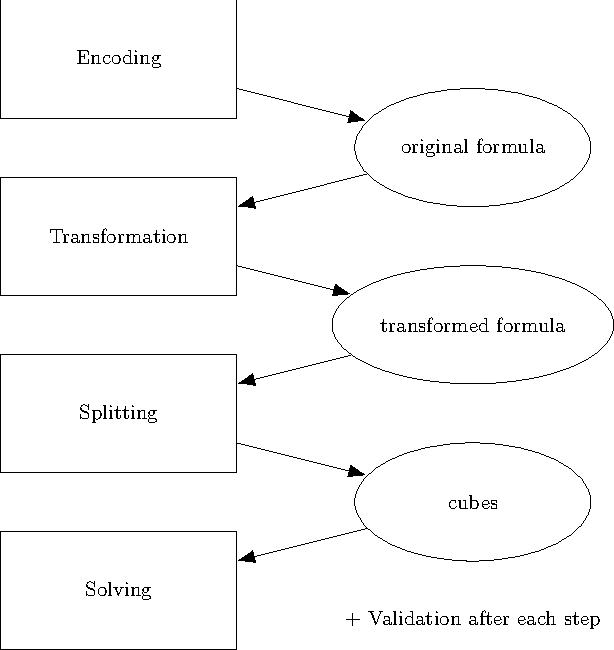
\includegraphics[scale=0.65]{images/framework}
	\end{figure}
\end{frame}

\section{Encoding}

\begin{frame}{Encoding}
	\begin{figure}
		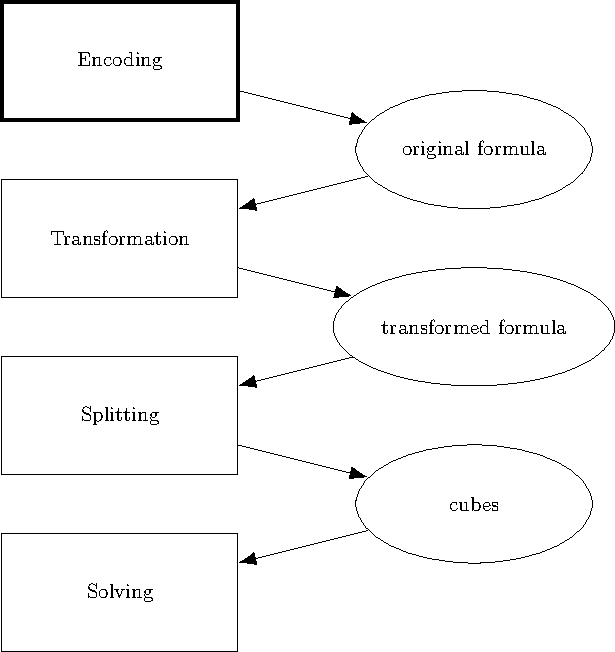
\includegraphics[scale=0.65]{images/framework1}
	\end{figure}
\end{frame}

\begin{frame}{Encoding - Intuition}
	Idea:
	\begin{itemize}
		\item one variable for each number
		\pause
		\item interpretation gives partition
		\pause
		\item one constraint clause for each Pythagorean triple
	\end{itemize}
\end{frame}

\begin{frame}{Encoding}
	Binary Pythagorean triple problem with $n$ numbers \\
	\vspace{5px}
	\pause
	Set of variables $V = \{ p_k \mid 1 \leq k \leq n \}$ \\
	\vspace{5px}
	\pause
	Constraint for non-equality: $NotEqual(x,y,z) = (x \vee y \vee z) \wedge (\neg x \vee \neg y \vee \neg z) $ \\
	\vspace{5px}
	\pause
	Constraint for all Pythagorean triples: $F = \bigwedge\limits_{x^2+y^2=z^2} NotEqual(p_x,p_y,p_z)$ \\
	\vspace{10px}
	\pause
	For an interpretation $I \subseteq V$ with $I \models F$, the resulting partition is:
	\begin{itemize}
		\item $ P_1 = \{ x \mid p_x \in I \}$
		\item $ P_2 = \{ x \mid p_x \notin I \} $
	\end{itemize}
\end{frame}

\begin{frame}{Encoding - Example}
	As in beginning example, $n=15$ \\
	\vspace{5px}
	\pause
	$V = \{ p_1, p_2, \dots ,p_{15} \}$
	\pause
	\begin{flalign*}
		F \quad = & \quad \quad (p_3 \vee p_4 \vee {\color<4->{ForestGreen}p_5}) \wedge ({\color<4->{ForestGreen}\neg p_3} \vee \neg p_4 \vee \neg p_5) &\\
		& \wedge \quad (p_6 \vee p_8 \vee {\color<4->{ForestGreen}p_{10}}) \wedge ({\color<4->{ForestGreen}\neg p_6} \vee \neg p_8 \vee \neg p_{10}) &\\
		& \wedge \quad (p_9 \vee p_{12} \vee {\color<4->{ForestGreen}p_{15}}) \wedge ({\color<4->{ForestGreen}\neg p_9} \vee \neg p_{12} \vee \neg p_{15}) &\\
		& \wedge \quad (p_5 \vee p_{12} \vee {\color<4->{ForestGreen}p_{13}}) \wedge (\neg p_5 \vee {\color<4->{ForestGreen}\neg p_{12}} \vee \neg p_{13}) &
	\end{flalign*}
	
	\pause
	Possible interpretation: $I = \{p_5, p_{10}, p_{13}, p_{15}\}$ \\
	\vspace{5px}
	\pause
	Resulting partition:
	\begin{itemize}
		\item $P_1 = \{1,2,3,4,6,7,8,9,11,12,14\}$
		\item $P_2 = \{5,10,13,15\}$
	\end{itemize}
\end{frame}

\section{Transformation}

\begin{frame}{Transformation}
	\begin{figure}
		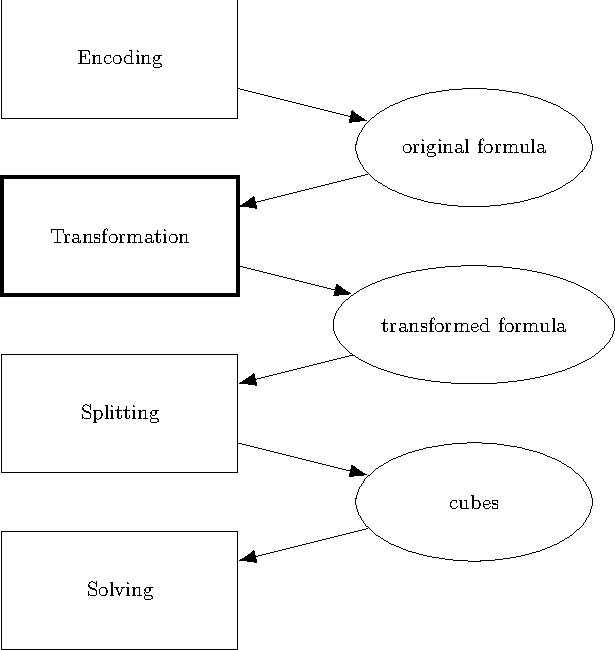
\includegraphics[scale=0.65]{images/framework2}
	\end{figure}
\end{frame}

\begin{frame}{Transformation}
	Goal: from $F$, find formula $F'$ which
	\begin{itemize}
		\item is easier to solve
		\pause
		\item preserves satisfiability
		\pause
		\item has models that can be easily transformed into models for $F$
	\end{itemize}
	\vspace{5px}
	\pause
	Approaches:
	\begin{itemize}
		\item eliminate some particular clauses
		\pause
		\item break partition symmetry
	\end{itemize}
\end{frame}

\begin{frame}{Clause elimination}
	\begin{flalign*}
		F \quad = & \quad NotEqual(p_3,p_4,p_5) &\\
		\wedge & \quad NotEqual(p_6,p_9,p_{12}) &\\
		\wedge & \quad NotEqual(p_9,p_{12},p_{15}) &\\
		\wedge & \quad NotEqual(p_5,p_{12},p_{13}) &
	\end{flalign*}
	Note $p_3$ only occurs in $NotEqual(p_3,p_4,p_5)$ and thus does not affect any other clauses
	\vspace{5px}
	\pause
	\begin{itemize}
		\item if $p_4^I \neq p_5^I$ then $NotEqual(p_3,p_4,p_5)$ is satisfied
		\pause
		\item if $p_4^I = p_5^I = \top$ then $p_3^I = \bot$
		\pause
		\item if $p_4^I = p_5^I = \bot$ then $p_3^I = \top$
	\end{itemize}
	\vspace{5px}
	\pause
	$\rightarrow$ clause $NotEqual(p_3,p_4,p_5)$ will not cause conflict
	\vspace{5px}
	\pause
	\begin{itemize}
		\item remove $NotEqual(p_3,p_4,p_5)$ from $F$ to obtain $F'$
		\pause
		\item interpretation of $p_3$ is important but not represented in $F'$
		\pause
		\item $\rightarrow$ remember deleted clauses and modify interpretation of $F'$ accordingly
	\end{itemize}
\end{frame}

\begin{frame}{Clause elimination - Example}
	\begin{flalign*}
		F' \quad = & \quad NotEqual(p_6,p_9,p_{12}) &\\
		\wedge & \quad NotEqual(p_9,p_{12},p_{15}) &\\
		\wedge & \quad NotEqual(p_5,p_{12},p_{13}) & \\
		F \quad = & \quad F' \wedge NotEqual(p_3,p_4,p_5) &
	\end{flalign*}
	\vspace{5px}
	\pause
	Possible Interpretation: $I = \{p_6, p_{12}\}$ \\
	\vspace{5px}
	\pause
	$I \models F'$ but $I \not\models F$ \\
	\vspace{5px}
	$\rightarrow$ account for deleted constraint $NotEqual(p_3,p_4,p_5)$ \\
	\vspace{5px}
	\pause
	As $p_4^I = p_5^I = \bot$ we modify $p_3^I = \top$ \\
	\vspace{5px}
	\pause
	$I' = \{p_3, p_6, p_{12}\}$ \\
	\vspace{5px}
	$I' \models F$
\end{frame}


\begin{frame}{Breaking Symmetry}
	\begin{itemize}
		\item formulas $F$ and $F'$ are symmetric
		\pause
		\item if $I \models F'$ then $V \setminus I \models F'$
		\pause
		\item $\rightarrow$ introduce unit clause for variable $p_x$ occurring in $F'$
		\item $F'' = F' \wedge p_x$
	\end{itemize}
	\vspace{5px}
	\pause
	Note that every model for $F''$ is a model for $F'$ and the transformation is satisfiability preserving
\end{frame}


% Tobias' part
\section{Cube-and-conquer solving}

\begin{frame}{Splitting}
	\begin{figure}
		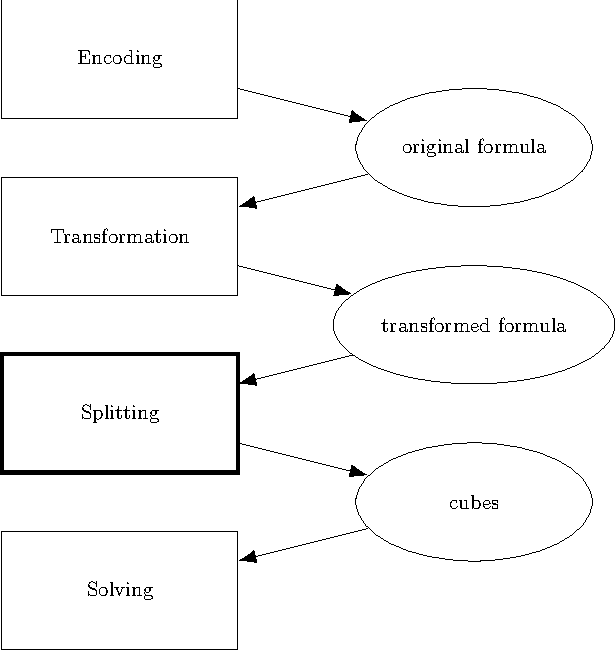
\includegraphics[scale=0.65]{images/framework3}
	\end{figure}
\end{frame}

\begin{frame}{Cube-and-conquer solving}
	\begin{itemize}
		\item Problem: solving with conflict-driven clause learning (CDCL) is too slow
		\pause
		\item Solution: 
		\begin{itemize}
			\item use different heuristics $\Rightarrow$ cube-and-conquer solver 
			\visible<6->{\item use parallelization (800 cores)}
		\end{itemize}
		% look-ahead heuristics
	\end{itemize}
	\pause

	\begin{figure}
		
		\begin{tikzpicture}
		% nodes
		\filldraw
		(5,0)  node[circle,inner sep=1pt,draw, fill=white](x5) {$x_5$};
		
		\filldraw 
		($(x5) + (-2, -1)$) node[circle,inner sep=1pt,draw, fill=white](x21) {$x_2$};
		\filldraw
		($(x5) + (2, -1)$) node[circle,inner sep=1pt,draw, fill=white](x7) {$x_7$};
		\filldraw
		($(x21) + (-1, -1)$) node[circle,inner sep=1pt,draw, fill=white](x3) {$x_3$};
		\filldraw
		($(x21) + (1, -1)$) circle (3pt) node[below] {$\bigwedge $} coordinate(p3);
		\filldraw
		($(x3) + (-0.75, -0.75)$) circle (3pt) node[below] {$\bigwedge $} coordinate(p1);
		\filldraw
		($(x3) + (0.75, -0.75)$) circle (3pt) node[below] {$\bigwedge $} coordinate(p2);
		
		\filldraw
		($(x7) + (-1, -1)$) node[circle,inner sep=1pt,draw, fill=white](x22) {$x_2$};
		\filldraw
		($(x7) + (1, -1)$) node[circle,inner sep=1pt,draw, fill=white](x6) {$x_6$};
		\filldraw
		($(x22) + (-0.75, -0.75)$) circle (3pt) node[below] {$\bigwedge $} coordinate(p4);
		\filldraw
		($(x22) + (0.75, -0.75)$) circle (3pt) node[below] {$\bigwedge $} coordinate(p5);
		\filldraw
		($(x6) + (0.75, -0.75)$) node[circle,inner sep=1pt,draw, fill=white](x23) {$x_2$};
		\filldraw
		($(x6) + (-0.75, -0.75)$) circle (3pt) node[below] {$\bigwedge $} coordinate(p6);
		\filldraw
		($(x23) + (-0.75, -0.75)$) circle (3pt) node[below] {$\bigwedge $} coordinate(p7);
		\filldraw
		($(x23) + (0.75, -0.75)$) circle (3pt) node[below] {$\bigwedge $} coordinate(p8);
		
		
	
		% edges
		\draw[] (x5) -- node[above] {\bf t} (x21);
		\draw[] (x5) -- node[above] {\bf f} (x7);
		
		\draw[] (x21) -- node[above] {\bf t} (x3);
		\draw[] (x21) -- node[above] {\bf f} (p3);
		
		\draw[] (x3) -- node[above] {\bf t} (p1);
		\draw[] (x3) -- node[above] {\bf f} (p2);
		
		\draw[] (x7) -- node[above] {\bf t} (x22);
		\draw[] (x7) -- node[above] {\bf f} (x6);
		
		\draw[] (x22) -- node[above] {\bf t} (p4);
		\draw[] (x22) -- node[above] {\bf f} (p5);
		
		\draw[] (x6) -- node[above] {\bf t} (p6);
		\draw[] (x6) -- node[above] {\bf f} (x23);
		
		\draw[] (x23) -- node[above] {\bf t} (p7);
		\draw[] (x23) -- node[above] {\bf f} (p8);
		
		\begin{pgfonlayer}{bg}
		
		\visible<6->{
			\draw [draw=OrangeRed1, line width=2pt] plot [smooth ,tension=0.75]coordinates { 
				($(x21) + (-2,0)$)
				(x21) 
				(x22)
				(x6)
				($(x6) +(1.5, 0.25)$)
			};
		}
		\visible<4->{
			\draw [draw=mdwblue, line width=2pt] plot [smooth ,tension=0.75]coordinates { 
				($(p1) + (-0.5, 0)$)
				(p1)
				(p2)
				(p3)
				(p4)
				(p5)
				(p6)
				(p7)
				(p8)
				($(p8) + (0.5, 0)$)
			};
		}
		\end{pgfonlayer}

		% captions
		\visible<4-3>{\node(look-ahead1) at ($(x5) + (-4.5, 0)$){\textbf{look-ahead}}; }
		\visible<6->{\node[text = OrangeRed1, align=center](3000) at ($(look-ahead1) + (-1, -1.2)$){\bf $\approx$ 3000 \\ \bf binary clauses};}
		\visible<5-5>{\node(look-ahead2) at ($(look-ahead1) + (0, -1.5)$){ \bf look-ahead};}
		\visible<4->{\node[text = mdwblue, align = center](3450) at ($(look-ahead2) + (-1, -1.25)$){\bf 3450 unassigned\\ \bf variables};}
		\visible<5-5>{\node(CDCL) at ($(look-ahead2) + (0, -2)$){\bf CDCL};}

		\end{tikzpicture}
		%\caption{Binary branching tree}
		
	\end{figure}
 \end{frame}



\section{Conclusion}

\begin{frame}{Solving}
	\begin{figure}
		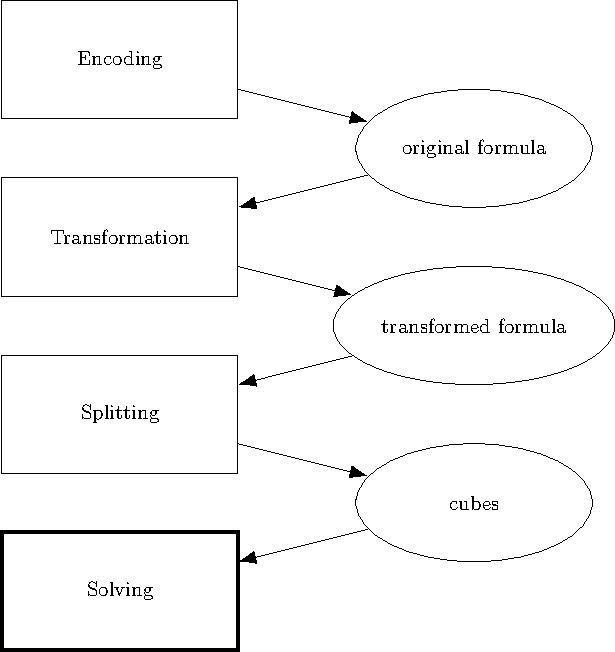
\includegraphics[scale=0.65]{images/framework4}
	\end{figure}
\end{frame}


\begin{frame}{Runtime}
	\begin{itemize}
		\item Splitting: 22000 CPU hours 
		\item Solving: 13000 CPU hours 
		\item Validation: 16000 CPU hours 
		\item sums up to $\approx$ 5.8 CPU years
	\end{itemize}
	\pause
	\begin{figure}
		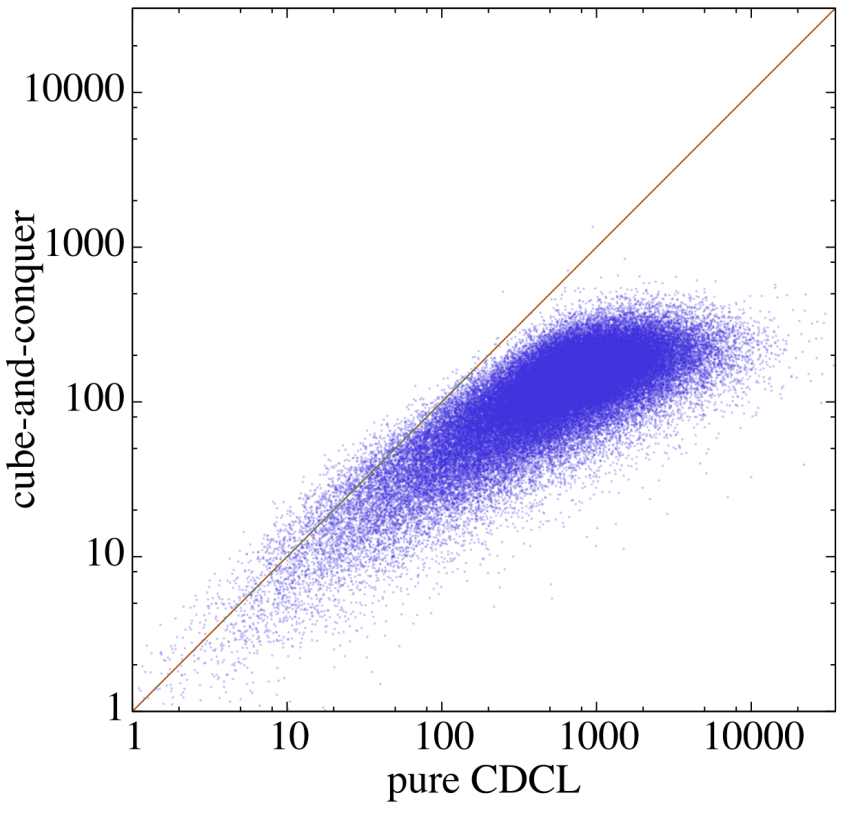
\includegraphics[width=0.5\textwidth]{images/plot1.png} 
		%\caption{runtime of C\&C and CDCL}
	\end{figure}
\end{frame}

\begin{frame}{Solution}
\begin{figure}
	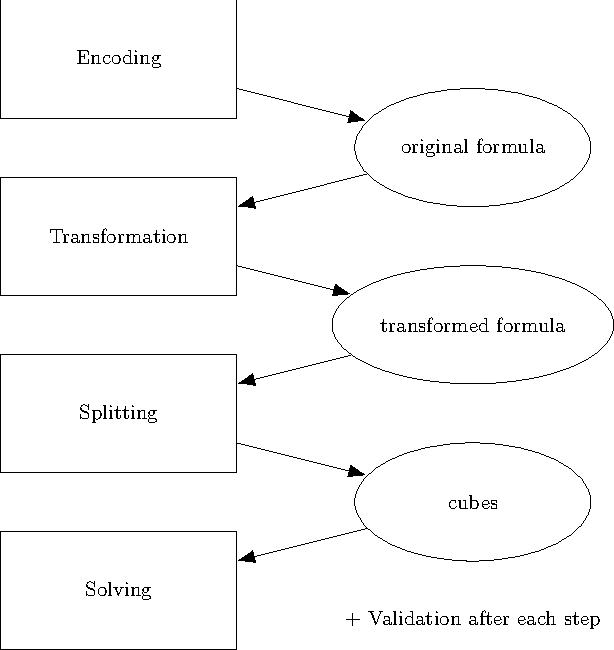
\includegraphics[scale=0.65]{images/framework}
\end{figure}
\end{frame}

\end{document}
